\documentclass[10pt,journal,compsoc]{IEEEtran}

\usepackage{verbatim}
\usepackage{url}
\usepackage{graphicx}

\usepackage{xspace}
\newcommand{\FC} {Freechains\xspace}

\newcommand{\Xon} {$1{\rightarrow}N$\xspace}
\newcommand{\Xno} {$1{\leftarrow}N$\xspace}
\newcommand{\Xnn} {$N{\leftrightarrow}N$\xspace}
\newcommand{\Xoo} {$1{\leftrightarrow}1$\xspace}
\newcommand{\Xo}  {$1{\hookleftarrow}$\xspace}

\begin{comment}
- content                                                                       
- CPU work to create blocks, easy objective verification, 50+1 attack, collapse
- Human work to create content, easy subjective verification, 50+1 attack,
  community fork (actually encouraged)
- unique identity based on CPU
- here based on post quality
- not CDN: Content delivery network                                             

(b) double spend of coins/reps is solved by total ordering all
Users can like \& dislike posts, which transfer reputation between them.
Reputation is created from news

Just like Bitcoin reaches consensus with the longest chain
uses mining to

(excess, SPAM, fake, abuse, illegal)                                            
\end{comment}

\begin{document}
\title{
    Peer-to-Peer Content Consensus based on Authoring Reputation
}
\author{
    Francisco Sant'Anna~\IEEEmembership{Department of Computer Science, Rio de Janeiro State University}
}

\IEEEtitleabstractindextext{%
\begin{abstract}
Content publishing in public Internet forums and social media suffer from
excess and abuse, such as low quality posts and fake news.
Centralized platforms employ filtering algorithms and anti-abuse policies, but
impose full trust from users.
We propose a publish-subscribe peer-to-peer protocol to model public content
dissemination without centralized control.
The central idea of the protocol is a reputation system that moderates content
and, at the same time, reaches network consensus.
We trace a parallel with Bitcoin:
    consolidated posts create reputation (vs proof-of-work);
    likes and dislikes transfer reputation (vs transactions);
    and forks are ordered by reputation (vs longest chain).
The reputation system depends solely on human work to create and rate content,
preventing content excess and abuse and imposing consensus on a peer-to-peer
setting.
\end{abstract}

\begin{IEEEkeywords}
peer-to-peer, consensus, reputation system, publish-subscribe
\end{IEEEkeywords}}

\maketitle

\section{Introduction}
\label{sec.introduction}

\IEEEPARstart{C}{ontent} publishing, such as in public Internet forums and
social media platforms, is increasingly more centralized in the hands of a few
companies~\cite{internet.fixing}.
%
On the one hand, these companies offer friendly user interfaces, free storage,
and permanent connectivity.
On the other hand, they concentrate more power than required to operate, since
they collect and control our data, ``algorithmize'' our consumption, and yet
obstruct portability with proprietary standards.
%
Peer-to-peer alternatives~\cite{p2p.survey} eliminate intermediates and push to
end users the responsibility to manage data and connectivity.
Due to decentralization of authority and network infrastructure, some new
challenges arise to deal with malicious users, support content discovery, and
enforce overall state consistency.

In a scenario of interest, suppose users want to discuss a political event by
posting public comments in the network.
In an ideal system,
(i)   all posts would eventually reach all users, even those temporarily
      disconnected;
(ii)  posts would be delivered to users in a consistent order;
(iii) the interactions among users would be respectful and on topic.
In a centralized system, items (i) and (ii) are trivially achieved assuming
availability and delivery order in the service, while for item (iii) users must
trust the service to moderate content (e.g., removing SPAM and fake news).
In a decentralized setting, however, none of these demands are easily
accomplished.
A common approach in gossiping protocols is to replicate the whole conversation
in all peers and disseminate proactively until all users receive
it.~\cite{p2p.survey}
However, this approach does not guarantee consensus since posts can be received
in conflicting orders in different peers.
As an example, antagonistic messages such as \emph{"X is decided"} vs
\emph{"Y is decided"} might be sent concurrently, preventing the network to
decide as a group between \emph{X} and \emph{Y}.

Bitcoin~\cite{p2p.bitcoin} proposes the first successful permissionless
consensus protocol around scarce virtual assets, the \emph{bitcoin tokens},
which can be transferred between users.
%
The only way to create new tokens is to work towards consensus in the network
by proposing a total order among all transactions in the system.
The more CPU work is done, the stronger becomes the proposal, the more peers
follow it, the more tokens are mined.
There is a strong association between work, profit and consensus that enables
Bitcoin as a peer-to-peer cash system.
%
Bitcoin prevents the double-spending problem~\cite{p2p.bitcoin}, which is
analogous to conflicting posts in public discussions: deciding between \emph{X}
and \emph{Y} as a group is the same as trying to buy \emph{X} and \emph{Y} with
insufficient funds for both.
%
However, Bitcoin's basic operation is to blindly transfer tokens between users,
with no subjective judgment that could affect transactions.
In contrast, our challenge is on assessing human content based on social
interactions between them.

In this work, we propose a consensus algorithm based on authoring reputation.
Inspired by Bitcoin, content authors accumulate tokens named \emph{reps}, which
serve as currency to rate posts and users in the network.
Users can rate posts with likes and dislikes, which transfer \emph{reps}
between them.
In the algorithm, work is manifested as new posts, which reward authors with
\emph{reps}, but which are still judged by other users.
This way, like Bitcoin, token generation is expensive, while verification is
cheap and made by multiple users.
However, unlike Bitcoin, both creation and verification are subjective, based
on human creativity and judgement, which match our target domain of content
publishing.
Posts and likes are linked as blocks in a Merkle~DAG that persists the whole
conversation and is disseminated in the network.
To reach consensus, branches with more reputed authors (i.e., with more work)
take priority.
Conflicting operations in concurrent branches, such as likes with insufficient
\emph{reps}, are rejected along with further posts.
The proposed consensus algorithm is integrated in Freechains%
\footnote{\url{http://www.freechains.org}}~\cite{fcs.sbseg20},
a peer-to-peer publish-subscribe content dissemination protocol.

\begin{figure*}[ht]
\centering
%\includegraphics[width=\textwidth]{arranjos}
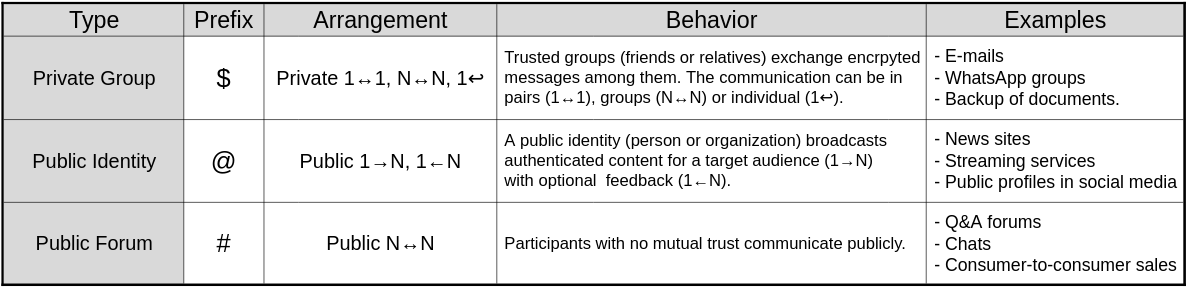
\includegraphics[width=\textwidth]{arrangements.png}
%\includegraphics[clip, trim=1.75cm 10.25cm 1.5cm 1.75cm, width=1.00\textwidth]{arranjos.pdf}
%\includepdf[width=\textwidth]{arranjos.pdf}
%\includepdf[pages=-,pagecommand={},width=\textwidth]{arranjos.pdf}
\caption{The three types of chains and arrangements in \FC.}
\label{fig.table}
\end{figure*}

In Section~\ref{sec.freechains}, we introduce the basic functionalities of \FC
to create and disseminate posts.
In Section~\ref{sec.consensus}, we describe the consensus algorithm with its
goals, incentives, and possible attacks and mitigations.
In Section~\ref{sec.related}, xxx.
In Section~\ref{sec.conclusion}, yyy.

\section{Freechains}
\label{sec.freechains}

\FC is an unstructured peer-to-peer topic-based publish-subscribe system.
Each topic, or \emph{chain}, is structured as a \emph{Merkle DAG}, i.e., a
directed acyclic graph immune to modifications.
The chain graph is disseminated peer by peer in the network with gossiping.
An author posts a message to a chain and all other users subscribed to the same
chain eventually receive the message.
\FC supports multiple types of chains with different arrangements of public and
private communication, which are detailed in Figure~\ref{fig.table}.
In this section, we describe the overall operation and structure of chains with
private groups, which are the simplest type of chains.
At the end of this section, we also illustrate public identity chains.
In Section~\ref{sec.consensus}, we detail the behavior of public forums, which
involve untrusted communication between users and require the proposed
reputation and consensus mechanisms.

All \FC operations go through a \emph{daemon} (analogous to Bitcoin full nodes)
which validates posts, links them in the Merkle DAGs, persists the chains in
the disk, and communicates with other peers in the network to disseminate the
graphs.
The command that follows starts a daemon to serve further operations:

{\footnotesize
\begin{verbatim}
 $ freechains-host start /var/freechains/
\end{verbatim}
}

The actual operations use a separate client software that communicates with the
daemon.
The next sequence of commands (i) creates a shared key, (ii) joins a private
group chain, and (iii) posts a message in the chain:

{\footnotesize
\begin{verbatim}
 $ freechains crypto shared "strong-password" # (i)
 A6135D..
 $ freechains "$family" join A6135D..         # (ii)
 42209B..
 $ freechains "$family" post "Good morning!"  # (iii)
 1_EF5DE3..
\end{verbatim}
}

\begin{figure}[t]
\centering
%\includegraphics[width=\textwidth]{arranjos}
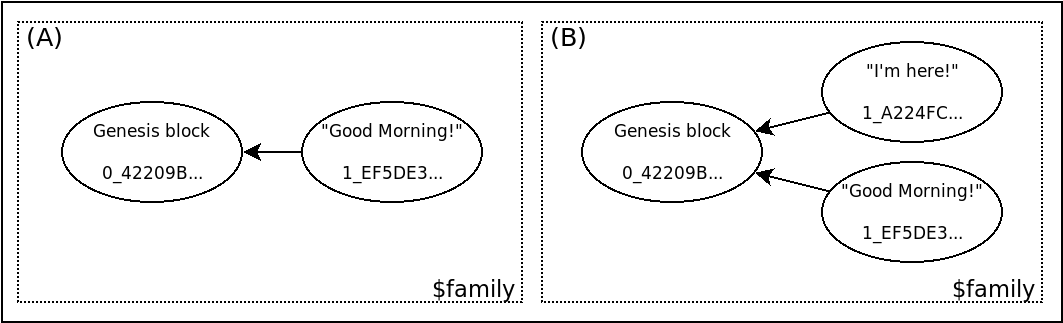
\includegraphics[width=0.5\textwidth]{family.png}
%\includegraphics[clip, trim=1.75cm 10.25cm 1.5cm 1.75cm, width=1.00\textwidth]{arranjos.pdf}
%\includepdf[width=\textwidth]{arranjos.pdf}
%\includepdf[pages=-,pagecommand={},width=\textwidth]{arranjos.pdf}
\caption{Two DAG configurations. (A) has a single head pointing to the
genesis block. (B) has a fork with two heads pointing to the genesis block.}
\label{fig.family}
\end{figure}

In the example, we join a private group chain (prefix $\$$) which stores and
transmits all messages encrypted.
A private chain requires that all participants use the same shared key when
joining the group.
A \emph{join} only initializes the DAG locally in the file system, and a
\emph{post} also only modifies the local structure.
No communication occurs at this point.
Figure~\ref{fig.family}.A depicts the state of the chain after the first post.
The genesis block with height $0$ and hash beginning with \texttt{42209B}
depends only on the arguments given to \emph{join}.
The next block with height $1$ contains the posted message, and its hash
\texttt{EF5DE3} depends on its payload and hash of its previous block,
complying with the Merkle~DAG.

\FC adheres to the \emph{local-first} software principle~\cite{p2p.local},
allowing that networked applications build on top of it to host their own data
and work locally while offline.
Except for synchronization, all other operations in the system only affect the
local replica.
In particular, joining a chain with the same arguments in another peer results
in the same genesis state, even if the peers have never met before.
Hence, before synchronizing, others peers have to initialize the chain with the
same steps:

{\footnotesize
\begin{verbatim}
 $ freechains-host start /var/freechains/
 $ freechains crypto shared "strong-password"
 A6135D..
 $ freechains "$family" join A6135D..
 42209B..
\end{verbatim}
}

Synchronization is explicit, in pairs, and unidirectional.
The next command asks daemon in \emph{localhost} to connect to daemon in
\emph{remote-ip} and receive all missing blocks from there:

{\footnotesize
\begin{verbatim}
 $ freechains "$family" recv <remote-ip>
 1/1 # one block received from <remote-ip>
\end{verbatim}
}

The command \emph{send} would synchronize the graph in the other direction.
Note that \FC does not construct a network topology or synchronize peers
automatically.
There are no preconfigured peers, no \emph{root servers}, no peer discovery.
All connections happen through the \emph{send} and \emph{recv} commands which
have to specify the peers explicitly.
In this sense, the protocol only gives basic support for communication in pairs
of peers and any further automation requires external tools.

The next sequence of commands checks the hash(es) of the block(s) at the head
of the graph (the latest blocks), and then reads the payload of the single head
found:

{\footnotesize
\begin{verbatim}
 $ freechains "$family" heads
 1_EF5DE3..
 $ freechains "$family" payload 1_EF5DE3..
 Good morning!
\end{verbatim}
}

Now the new peer is in the same state as the original peer in
Figure~\ref{fig.family}.A.
However, since the network is inherently concurrent and users are encouraged to
work locally, typical graphs are not lists, but DAGs with multiple heads.
As an example, suppose the new peer posts a new message "I'm here!" before the
\emph{recv} above, when the local graph is still in the genesis state.
In this case, the resulting graph after the synchronization, now would contain
two blocks with height $1$, as illustrated in Figure~\ref{fig.family}.B.

Forks create ambiguity when trying to order messages in a conversation.
In private chains, in which users trust each other, an external method for
consensus could be applied if necessary.
As a simple solution, users could rely on the timestamps of blocks to order all
messages in conversation.
However, in public chains, malicious users could modify their local time to
affect new block timestamps and manipulate the order of messages.
Furthermore, when we introduce the reputation system, conflicting \emph{like}
operations must be accounted directly by the protocol, since they affect the
reputation of users and may block certain posts.
For these reasons, we need an internal autonomous consensus algorithm.

For the sake of completeness, \FC also supports public identity chains (prefix
$@$), which relies on public-key cryptography to attach an identity to a chain
and to verify the authenticity of posts:

{\footnotesize
\begin{verbatim}
 $ freechains crypto pubpvt "strong-password"
 EB172E.. 96700A..
 $ freechains "@EB172E.." join
 F4EE21..
 $ freechains "@EB172E.." post "This is Pele" \
    --sign=96700A..
 1_547A2D..
\end{verbatim}
}

In the example above, the author \emph{Pel\'e} creates a pair of public-private
keys and joins an identity chain attached to his public key.
Then, he needs to sign every post with his private key to be accepted in the
network.

\section{Consensus Algorithm}
\label{sec.consensus}

Without any kind of moderation, public forums

{\footnotesize
\begin{verbatim}
 $ freechains "#chat" join "EB172E.."
 10AE3E..
 $ freechains "From Joe" --sign=96700A..
 1_547A2D..
\end{verbatim}
}

---the one with more work---prefixes the
sequence as a whole.

Our sequencing proposal is straightforward and compares the sum of \emph{reps}
accumulated in the past by the authors in pairs of concurrent branches.

Consensus is still required because like operations spend \emph{reps} that need
to be verified consistently by all peers in the network.
To verify operations in concurrent branches, the graph must be sequenced to
generate a total order between blocks.
Our sequencing proposal is straightforward and compares the sum of \emph{reps}
accumulated in the past by the authors in pairs of concurrent branches.
The branch with more reputation---the one with more work---prefixes the
sequence as a whole.
If the suffixed branch has a conflicting operation (e.g., a like from a user
without reputation), then this operation and all remaining blocks are removed
from the DAG.

\section{Related Work}
\label{sec.related}

\section{Conclusion}
\label{sec.conclusion}



With this design, we retarget  , the balance between work, profit and consensus also applies 

attack 50+1 but not as
cite local-first software

 (crypto proof \& authoring),
while verification is cheap


requires work but evaluation


, but
are evaluated by other user
The system also imposes incentives to rate posts and 

Unlike bitcoin

Since likes and dislikes spend reputation, \emph{creps} are scarce resources
Incentives to post and rate content.

There is a strong association between work, profit and consensus that enables
Bitcoin as a peer-to-peer cash system.

distinguish SPAM from legitimate
Another problem CPU



content.



 (e.g., posts on social media, public conversations
based on the reputation of users
in the network.


biggest difference:
work is subjective as is the evaluation by other users


 with consensus since
whoever proposes the ordering will choose one of the operations arbitrarily


 which is similar to the
example above (\emph{buy X} vs \emph{buy Y})

spent

with work



this gives consensus with total order, solves double spend, which is equivalent
to solving X/Y is decided above

we borrow token, scarcity


 that requires work to 
Only one purpose


- incentive
- security

- Last-Write-Wins

- just all tokens are the same, no subjective judgment, for example on why token is being transferred


 and xx timestamps.


 of the service and , and trust from users to deal

In a decentralized setting, 
    - spam
    - abuse
    - on topic
    - disconnections
    - order

Bitcoin

responses would




n user posts 

- discovery
- also consensus, ensure that participants receive all data in a consistent order
- bitcoin, discovery even disconnected, consensus, but not quality


Regardless of the Internet growth over the years,

\subsection{Subsection Heading Here}
Subsection text here.

\subsubsection{Subsubsection Heading Here}
Subsubsection text here.

\section{Conclusion}
The conclusion goes here.

\bibliographystyle{IEEEtran}
\bibliography{tpd-21}

\begin{IEEEbiography}{Michael Shell}
Biography text here.
\end{IEEEbiography}

\begin{IEEEbiographynophoto}{John Doe}
Biography text here.
\end{IEEEbiographynophoto}

\begin{IEEEbiographynophoto}{Jane Doe}
Biography text here.
\end{IEEEbiographynophoto}

\end{document}
